\subsection{Product perspective}
The product will be used by farmers, policy makers and agronomists.
\subsubsection{Scenarios}

\paragraph{Scenario 1 : Farmer registration}\mbox{} \\

Ishaan receives an e-mail from administration that redirects him to the DREAM website registration page. He registers by providing his email address, name, surname, farm name and finally location which he provides by means of the geo-tracking functionality of his smartphone. The system checks that the email address isn't already registered, then sends a validation email to Ishaan.

After validation, the system fetchs Ishaan's district and mandal, based on his location. It then displays rainfall conditions and predictions, respectively based on Ishaan's mandal and location, on the homepage of Ishaan. It then fetchs the policy makers corresponding to this area. The system sends a notification to the policy maker in charge of the area to acknowledge the registration of Ishaan.

\paragraph{Scenario 2 : Production data and type release}\mbox{} \\

Shyla has just finished his crop. She measures her production. She logs in on the DREAM platform where she had already registered. She goes to the page "Release production". She fills the following sections: seed variety, seed rate, production amount, surface area of the cultivated fields, amount of water consumed, start and end date.

\paragraph{Scenario 3 : Discussion forum creation}\mbox{} \\

Dhruv's old tractor is broken. He wonders if he should try to repair it, if possible, and if not, what modern model he should choose. He looks for feedbacks on the forum discussion of the DREAM platform. As he can't find any on the kind of engine he owns, he creates a new topic, explains his issue and waits for answers.

\paragraph{Scenario 4 : Prediction check}\mbox{} \\

Ashwin wants to know what are the soil and weather conditions of his mandal to correctly dose his fertilizer. He logs in on the DREAM platform. He goes to the homepage. He checks the soil moisture data, weather conditions and predictions.

\paragraph{Scenario 5 : Request for production data and type release}\mbox{} \\

Between April and October, Amar crops and harvests rice during the so-called "Kharif"season. In November, he receives a notification from DREAM that urges him to release his production data - seed variety, seed rate, production amount, surface area of the cultivated fields, amount of water consumed, start and end date - by the end of the month. He instantly performs. On the first of December, a notification telling the completeness of the database gathering the production data of the farmers in Amar's area based on the location of his farm is sent by the system to the dedicated policy maker.

\paragraph{Scenario 6 : Research among discussion forums}\mbox{} \\

Diya is not sure about the law regarding some specific fertilizer. She looks for discussion forums on DREAM. She uses as keywords "law", the name of the fertilizer and she filters the results to get late discussions - she knows that the law has changed in the previous years. She finds some farmer whose response handles her issue. Since she wants some more precision, she contacts the farmer, via DREAM, in a private discussion.

\paragraph{Scenario 7 : Help request notification}\mbox{} \\

Sahil receives a notification from his policy maker suggesting him some practices fertilizer,crops and overall practices to improve his productivity and a proposal for a specific help request.

\paragraph{Scenario 8 : Well performing farmers identification}\mbox{} \\

Nikhil is a policy maker. On December, 1st, he receives a notification from DREAM telling that all farmers of his area have delivered their production data. He selects some performance metrics among those proposed. The systems ranks the farmers accordingly and displays the ranking. Nikhil selects the farmer that he wants to congratulate. He sends to each one a message via DREAM, and ticks a box to send an e-voucher that the system generates and enclose. In the messages, Nikhil asks for best practices to the farmers.

\paragraph{Scenario 9 : Poorly performing farmers identification}\mbox{} \\
% del line : Based on the data of these farmers and figures of the previous years, the system computes the personalized suggestions to each of them (should/could it be computed ?) ????
Ananya is a policy maker. On December, 1st, she receives a notification from DREAM telling that all farmers of her area have delivered their production data. She selects some performance metrics among those proposed. The systems ranks the farmers accordingly and displays the ranking. Ananya selects the farmers that may require help. She sends them a message via DREAM to tell them these suggestions and propose them to be helped.

\paragraph{Scenario 10 : Major issues identification}\mbox{} \\

Nila is a policy maker. Crop is coming to end. She wants to correctly understand the issues that face the farmers of her area, in order to ask relevant questions to well performing farmers. She spends some time on forum discussions and note the most repeating concerns of farmers.

\paragraph{Scenario 11 : Help request}\mbox{} \\

Tamia requires the insight of some expert on crops for the coming seeding. She goes to the "help request" section. She sends message. Based on her location, the system forwards the message to the adequate policy maker. The latter will send the request to an agronomist, who will afterwards contact Tamia.

\subsubsection{Product functions}

\begin{itemize}
	\item
	R1: When a farmer asks for personalized suggestions, the system should retrieve the weather, soil and location data
	\item
	R2: If a farmer performs well, policy makers will request his best practices
	\item
	R3: At each end of cropping, the system should request production data of farmers.
	\item
	R4: The system fetches using external database the data about soil and irrigation
	\item
	R5: The system should compute the performance indicators based on the data provided by farmers
	\item
	R6: When a policy maker asks for poor-performing farmers, the system should retrieve the associated farmers.
	\item
	R7: When a policy maker asks for well-performing farmers, the system should retrieve the associated farmers.
	\item
	R8: The system should grant farmers access to their personal and production data
\end{itemize}

\subsubsection{Assumptions, dependencies and constraints}
%TODO
\begin{itemize}
	\item
	Cropping seasons are the same on the whole Telengana State and follow the Kharif/Rabi calendar, see Figure \ref{fig:seasons} % (see Recommended System of Breeder Seed Indent and Supply)
	\item
	Farmers put rightful information on their location and data on their production. Fraud is possible but it is the responsibility of policy makers to prevent it, with the help of agronomists.
	\item
	If a policy maker is missing at some farmer's registration, he/she will be found before the end of the cropping season.
	\item
	All farmers that register have access to internet in some way and have access to the application.
	\item
	All humidity data are collected through the database of the NICES project. The system thus doesn't require its own sensors.
	\item
	To avoid money transfers and check the use of the money, incentives are sent as e-vouchers.
	\item
	The irrigation system is supposed to provide the water consumption data thanks to an external API.
	
\end{itemize}

\begin{figure}[H]
	
	\centering
	
	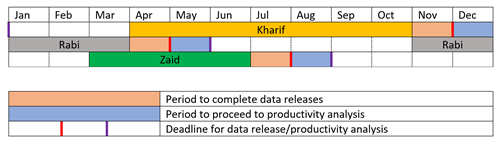
\includegraphics[width=\columnwidth]{Images/croping-seasons-calendar.png}
	
	\caption{Seasons}
	
	\label{fig:seasons}
	
\end{figure}


